% -----------------------------------------------
% Template for ISMIR 2010
% (based on earlier ISMIR templates)
% -----------------------------------------------

\documentclass{article}
\usepackage{ismir2010,amsmath,cite}
\usepackage{graphicx}
\usepackage{url}
\usepackage{algorithm,algorithmic}


% Title.
% ------
\title{Large-scale harmonic patterns clustering}

% Single address
% To use with only one author or several with the same address
% ---------------
%\oneauthor
% {Names should be omitted for double-blind reviewing}
% {Affiliations should be omitted for double-blind reviewing}

% Two addresses
% --------------
%\twoauthors
%  {First author} {School \\ Department}
%  {Second author} {Company \\ Address}

% Three addresses
% --------------
\threeauthors
  {First author} {Affiliation1 \\ {\tt author1@ismir.edu}}
  {Second author} {\bf Retain these fake authors in\\\bf submission to preserve the formatting}
  {Third author} {Affiliation3 \\ {\tt author3@ismir.edu}}
% what order do we use? Thierry, Ron, Dan?  Dan, Thierry, Ron?


\begin{document}
%
\maketitle
%
\begin{abstract}
The goal is to analyze very large collections of music. We describe
a clustering scheme of harmonic patterns that scales linearly in time
with the number of songs analyzed. These harmonic patterns are related
to the \textit{Shingles} idea, but we scale to larger sets and we do not
perform $k$-nn with them. We create a codebook and assert
its properties. In particular, we show that clustering with notions of
bars and song segments helps, and that we get codes associated more
with some artists than others.
\end{abstract}
%
\section{Introduction}\label{sec:introduction}


Large-scale \cite{Bertin-Mahieux2008}


\section{Previous Work}\label{sec:prevwork}
Casey and Slaney \cite{Casey2006,Casey2007,Casey2008}

\section{Data}\label{sec:data}
In this section we present our use of the Echo Nest features and the
datasets we use for training and testing our model.

\subsection{EchoNest API}


\subsection{USPOP}


\subsection{Artist Set}



\section{Algorithm}
Wth the scaling factor as our main concern, we present an online
vector quantization algorithm to cluster the harmonic patterns.

\begin{algorithm}
%\caption{Pseudocode of Vector Quantization}
\begin{algorithmic}
\STATE$l$ learning rate
\STATE$\{P_n\}$ set of patches
\STATE$\{C_k\}$ codebook of $K$ codes
%\STATE $m \leftarrow b$
\REQUIRE $0 < l \leq 1$
\FOR{$nIters$}
\FOR{$p \in \{P_n\}$}
\STATE$c \leftarrow min_{c \in C_k} dist(p,c)$
\STATE$c \leftarrow c + (p - c) * l$
\ENDFOR
\ENDFOR
\RETURN $\{C_k\}$
\caption{{Pseudocode of Online Vector Quantization. Note that we can replace
the number of iteration by a threshold on the distortion over some test set.}
\label{algo:vq}}
\end{algorithmic}
\end{algorithm}



\section{Experiments - Fundamentals}\label{sec:experiments}
Note that we will present two additional experiments in 
Section \ref{sec:exps2}.

\subsection{Basic Properties}
This section present some fundamental results of the clustering algorithm.
These are important, but do not change the larger picture. Thus we will not
spend too much time describing them. In short: more training samples is
better, more codes is better, larger patterns are more difficult.
\begin{itemize}
\item First, a larger dataset gives a better encoding codebook. See Figure
\ref{fig:data_sizes}.
\item Secondly, a larger codebook better encodes new song. See 
Table \ref{tab:cbsize}.
\item Finally, larger patterns are more difficult to encode, thus require
larger codebooks. See Figure \ref{fig:perbeat}.
\end{itemize}

These properties are important to verify and measure, but they are not
surprising for a clustering algorithm. We move on to more interestng facts.

\begin{figure}[htb]
\begin{center}
\includegraphics[width=.99\columnwidth]{data_sizes}
\end{center}
\caption{\small{Distortion for a codebook of size $100$ encoding one bar
at a time, a bar being represented by $4$ chroma feature vector.
Therefore, a code or a pattern is of size $12$ x $4$ = $48$.
Distortion measure on the test data set. Data size tested range
from $10$ thousands to $2$ millions. Patterns were selected at
random from the dataset of approximately $3,7$ million patterns.}}
\label{fig:data_sizes}
\end{figure}

% NEW RESULTS COMING SOON WITH FIXED SIZED DATASET
\begin{table}
\begin{center}
\begin{tabular}{|l|l|c|}
\hline
\# codes & \# samples & avg. dist \\ \hline \hline
1 & $500$ & $0.066079$ \\
10 & $5$K & $0.045690$ \\
50 & $25$K & $0.038456$ \\
100 & $50$K & $0.036725$ \\
200 & $100$K & $0.033923$ \\
500 & $250$K & $0.030973$ \\
1000 & $500$K & \\ \hline
\end{tabular}
\end{center}
\caption{\small{Experiment with the codebook size. We train on patterns
corresponding to $1$ bar resized to $4$ beats. The number of training
samples is set to $500$ times the number of codes, which is sufficient
according to Figure \ref{fig:sizes}. NEW RESULTS COMING SOON WITH FIXED 
SIZED DATASET }}
\label{tab:cbsize}
\end{table}


\begin{figure}[htb]
\begin{center}
\includegraphics[width=.9\columnwidth]{encoding_per_beat}
\end{center}
\caption{\small{Encoding larger and larger patterns with a fixed size
codebook.}}
\label{fig:perbeat}
\end{figure}

\subsection{Music Randomness}
It will not surprise any reader, music is not random. This fact should
become apparent in our experiments in the following way. Information
theory tells us that if the signal to encode doubles, we need to square
the size of the codebook to encode it with the same distortion.

To help the intuition, here is an example. Imagine a binary array of 
length $1$. We need two
codes to encode perfectly: $(0)$ and $(1)$. If the binary array is now of
length $2$, we now need four codes: $(0,0)$, $(0,1)$, $(1,1)$ and $(1,0)$.

Since music is not random, we expect that squaring the codebook when the
pattern size doubles will rather give improved results than constant ones.
See Figure \ref{it's comng...}.


\section{Visualization}
The goal here is to give an intuition to the reader of what kind of
typical patterns do we get. We also want to have a feel for what the
clusters look like, how many boring sustaned notes are encoded in the
codebook, can the codebook describes the complexity of the music space, etc.

Below we present some figures to help the reader with those questions.
Please keep in mind the limited space.

\subsection{Encoding of a Song}
Here we present a song with its two encodings. First, the harmonic patterns
given by the EchoNest. Secondly, each pattern is encoded by its closest
code in the codebook. See Figure \ref{fig:encodesong}.

\begin{figure}[htb]
\begin{center}
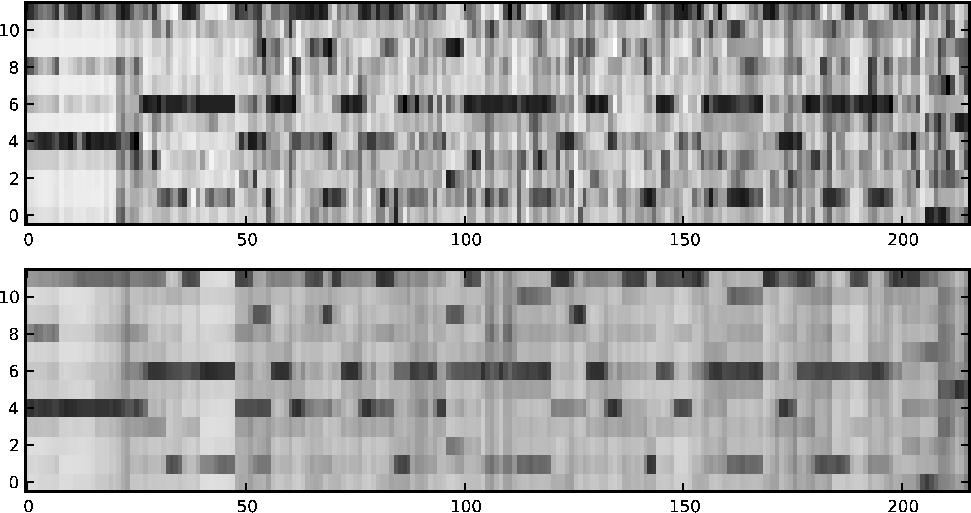
\includegraphics[width=.9\columnwidth]{song_encoded}
\end{center}
\caption{\small{Original song and its encoding. Must get a better one for
the paper!!!!!!}}
\label{fig:encodesong}
\end{figure}

\subsection{Codebook}
We can present the most typical patterns (Figure \ref{fig:codes1}). 
Then, LLE? (Figure \ref{fig:lle}). 
Then, the graph on variance. (Figure \ref{fig:code_var}).

\begin{figure}[htb]
\begin{center}
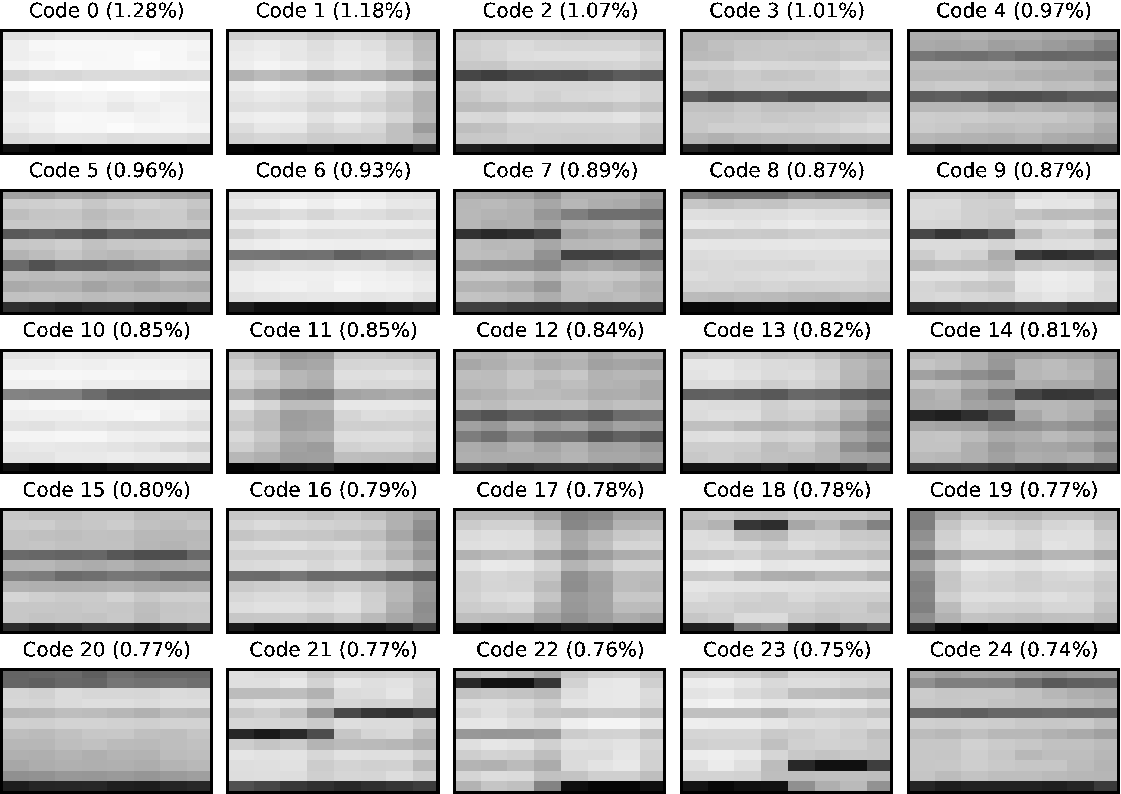
\includegraphics[width=.9\columnwidth]{codes1}
\end{center}
\caption{\small{Most used codes in the codebook.}}
\label{fig:codes1}
\end{figure}

\begin{figure}[htb]
\begin{center}
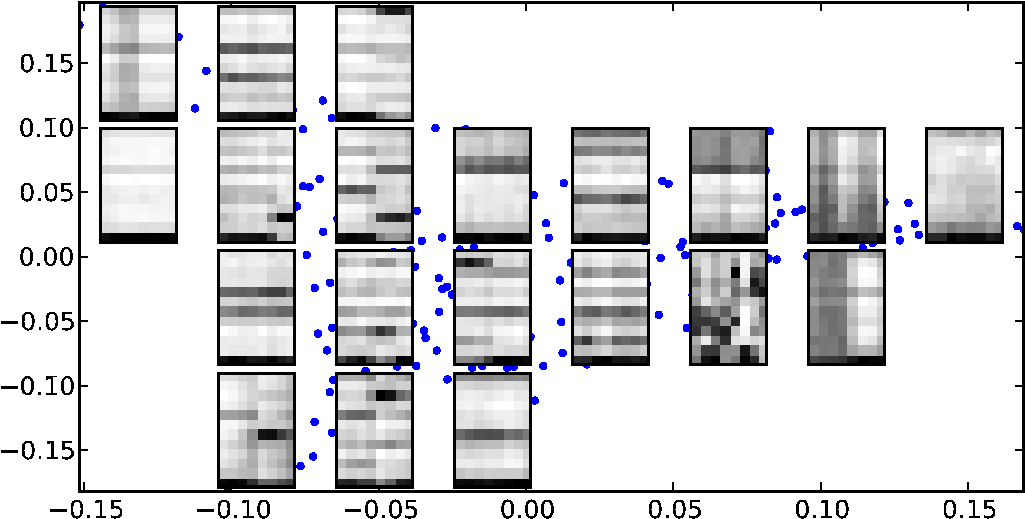
\includegraphics[width=.9\columnwidth]{codes_lle}
\end{center}
\caption{\small{Locally linear embedding (LLE) visualization of the codebook.}}
\label{fig:lle}
\end{figure}

\begin{figure}[htb]
\begin{center}
\includegraphics[width=.9\columnwidth]{code_variance}
\end{center}
\caption{\small{Average variance in time of a codebook.}}
\label{fig:code_var}
\end{figure}

\subsection{Cluster}
Here we present real patterns that are closer to the code presented in ...
than any other code. The goal is to feel how much variance is present in
a cluster. See Figure \ref{fig:cluster}.

\begin{figure}[htb]
\begin{center}
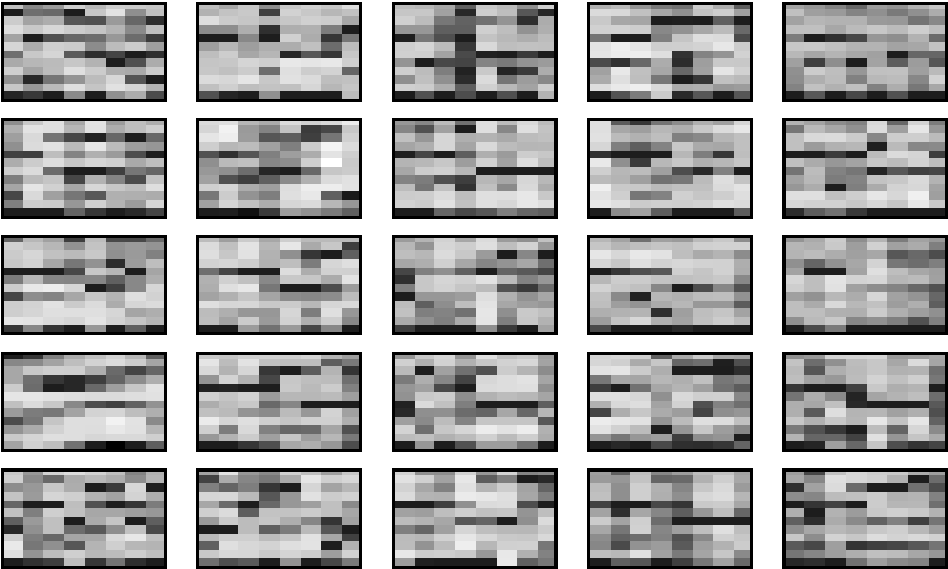
\includegraphics[width=.9\columnwidth]{close_patterns1}
\end{center}
\caption{\small{Cluster around some pattern... TO BE REDONE}}
\label{fig:cluster}
\end{figure}

\section{Further Experiments}\label{sec:exps2}

\subsection{Song Segmentation}
We explained that we used bars as defined by the EchoNest algorithm to
train our patterns. Let's assume once again that those bars are
reasonable. We investigate whether we could recover the bar segmentation
of new songs from our codebook. It would helps us assert that codes
encodes something related to bars, for instance a strong beat at the
beginning.

See Table \ref{tab:offset}.

\begin{table}
\begin{center}
\begin{tabular}{c|c}
%\hline
offset & \% of times chosen \\ \hline
0 & $\mathbf{62.6}$\\
1 & $16.5$\\
2 & $09.4$\\
3 & $11.5$\\
\end{tabular}
\end{center}
\caption{\small{
Best offset according to our codebook. The real one is $0$.
}}
\label{tab:offset}
\end{table}

\subsection{Artist Recognition}
Let us be clear, the clustering method proposed in this work is not
intended to perform well at artist recognition. An obvious fact is that
we lose all timbral information which would be usefull. However, we can
imagine that some artist use more often some patterns than others.
See Figure \ref{fig:conf_mat}.

\begin{figure}[htb]
\begin{center}
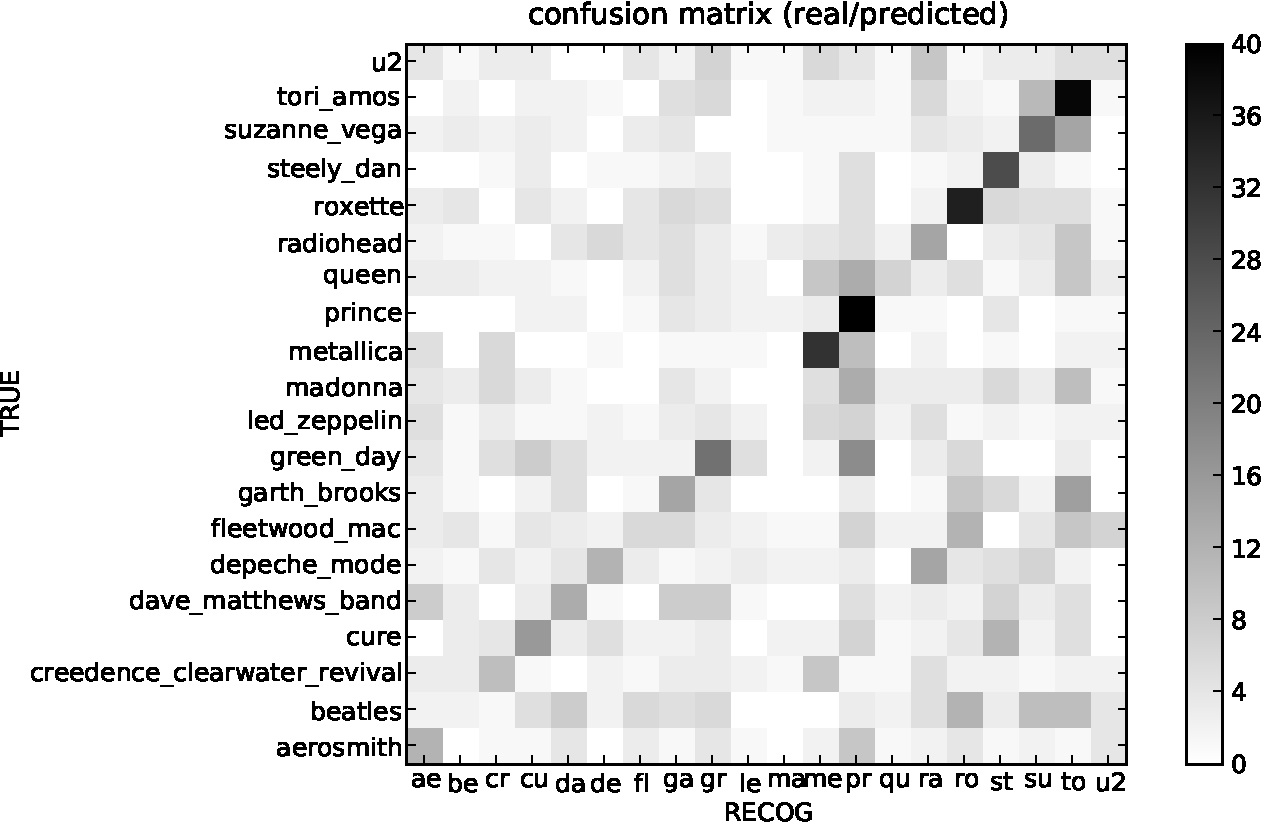
\includegraphics[width=.9\columnwidth]{conf_mat_per_artist}
\end{center}
\caption{\small{Confusion matrix for artist recognition task.}}
\label{fig:conf_mat}
\end{figure}

Looking at the most typical patterns per artist can be insightful.
To find these patters, we compare its use by one artist and divide
by its use by all artists. In Figure \ref{fig:metallica} we see 
Metallica's pattern and in Figure \ref{fig:amosvega}, Tori Amos and
Suzanne Vega's pattern. These three artists were easily identified.

\begin{figure}[htb]
\begin{center}
\includegraphics[width=.4\columnwidth]{metallica_pattern}
\end{center}
\caption{\small{Most typical pattern for Metallica.}}
\label{fig:metallica}
\end{figure}

\begin{figure}[htb]
\begin{center}
\includegraphics[width=.4\columnwidth]{toriamos_suzannevega_pattern}
\end{center}
\caption{\small{Most typical pattern for Tori Amos and Suzanne Vega.}}
\label{fig:amosvega}
\end{figure}



\section{Conclusion and Future Work}


\small
%\section{Acknowledgements}
%Thierry is NSERC graduate fellow, or some title like that.
% Graham for the NMF stuff, unless is an author.

%\begin{thebibliography}{citations}
%\bibitem{Someone:04} 
%X. Someone and Y. Someone:
%{\it Title of the Book},
%Editorial Acme, Utrecht, 2004.
%\end{thebibliography}

\bibliography{tbm_bib}





\end{document}
